% TODO: ПОМЕНЯЙТЕ НА СВОЙ ПУТЬ ПРИ СБОРКЕ
\renewcommand{\mainFolder}{/home/aleksei/github_projects/latex_works/informatics/3sem}
\renewcommand{\myFolder}{\mainFolder/lecture_\arabic{lectureNo}/}

%	LECTURE INFO
%----------------------------------------------------------------------------------------
\renewcommand{\lectureSubject}{Введение в C++}
%----------------------------------------------------------------------------------------
%
% Главное - указывать в путях для добавляемых файлов переменную \myFolder.
% Так, новый cpp файл должен иметь путь \cppfile{\myFolder/main}{....} (указывается без расширения)
% Нельзя писать \cppfile{main}{...} !!!
% Если не выполнить это требование, большой проект не будет собираться


\begin{lecture}[\lectureSubject]
	\begin{lecSection}[Этапы компиляции]
		C$++$ --- компилируемый язык. Перевод с человеческого языка на машинный код происходит не во время исполнения, а заранее. Сборка программы при этом проходит в несколько этапов:
		\begin{enumerate}
			\item \underline{Препроцессинг}: my.cpp $\rightarrow$ my.cpp$'$ \\
			Здесь происходит подстановка всех макросов, а акже удаление комментариев:
			\cppfile{\myFolder/macros}{Пример макроса}{1}
			\item \underline{Компиляция}: my.cpp$'$ $\rightarrow$ main.o \\
			Он содержит переведенную на машинный код инструкции, но все еще содержит сигнатуру функций. Это означает, что объектный файл может содержать названия функций, их входные данные, но не саму реализацию.
			\item \underline{Компоновка} (линковка): my.o $\rightarrow$ my.exe \\
			Здесь уже все файлы связываются и функции, не реализованные в п.3, получают реализацию. Программа может быть разделена на модули так, что разные файлы используют функции других файлов. При этом, если один файл ссылается на ресурсы других файлов, эти ресурсы необходимо объявить в отдельном файле: header--файле (хидер на жаргоне). Хидер содержит лишь сигнатуры функций и переменных, однако не входит в не конечный результат компиляции. Во время компановки эти хидеры будут показывать, где искать функции.\\
			Подобное деление лежит в основе принципа раздельной компиляции: программы делятся на компоненты, которые собираются по отдельности. Это уменьшает время компиляции.
		\end{enumerate}
	\end{lecSection}
	\begin{lecSection}[Синтаксис]
		\cppfile{\myFolder/skel}{Демонстрация синтаксиса}{ex1}
		В языке С$++$ есть особенности, отличающие его от Python. Так, при создании переменной необходимо явно указать ее тип (строка 4).\\
		В первой строке --- подключение библиотеки для работы ввода/вывода.\\
		В строке 5 стоит оператор ввода из стандартного ввода (это консоль) и спец. оператор $>>$. Результат считывания уходит в переменную x. std --- это пространство имен, о них будет сказано позже. \\
		В строке 6 --- вывод, по аналогии с вводом. При этом строки можно выводить конвейером (как видно `cout $<<$ "x=" $<<$ x` --- эти строки будут сшиты при выводе).\\
		В С$++$ табуляция не имеет значения, перевод строки после (6) и дальнейшие команды показывают это. \\
		Строка 8 содержит код возврата --- он будет возвращен по окончании программы (0 означает успех).
		 
	\end{lecSection}
	\begin{lecSection}[Арифметические операции и сравнение]
		x = y --- арифметическая операция (не присваивание, как в питоне). Можно писать такой код
		\cppfile{\myFolder/ariph}{Неясное поведение}{ariph_hack}
		В коде выше все работает, однако такое поведение программы будет неочевидным.
		В С$++$ все еще работают x $+$= 1. Помимо этого имеются два оператора: x$++$ $\approx$ $++$x $\approx$ x$+$=1.
		Разница следующая: y = (x$++$) запишет в y \textbf{старый} х, в то время как в y=($++$x) будет записан \textbf{новый} х. Операции ** (возведение в степень) \textit{нет}. Примеры некоторых арифметических действий:
		\begin{enumerate}
			\item x*y --- при применении к целым числам результат будет целым числом.
			\item x/y --- при применении к целым числам будет применено \underline{целочисленное} деление. Проблему можно решить, если добавить в конце ".". Так, $2/3$ станет $2/3.$ --- точка превратит число в вещественное.
			\item x $>$ y, x $>$= y, x == y. Это тоже арифметические операции, возвращают, правда, значение типа \textit{bool}: \textbf{true} или \textbf{false}.
		\end{enumerate}
	\end{lecSection}
	\begin{lecSection}[Циклы, условия и конструкции]
		В С$++$ три вида циклов, их синтаксис отличается от Python:
			\cppfile{\myFolder/c1}{Виды циклов}{c1}
			Условие надо обязательно кидать в скобки, иначе С$++$ не сможет отличить его от тела.
			\cppfile{\myFolder/c2}{Виды циклов}{c2}
			Здесь мы выходим из цикла по команде \textbf{break}.
			\cppfile{\myFolder/c3}{Виды циклов}{c3}
			Как обычный while, но сначала выполняет тело цикла, а затем проверяет условие.
			\cppfile{\myFolder/c4}{Виды циклов}{c4}
			Это очень похоже на то, что в питоне было под видом
			\pythonfile{\myFolder/py_example1}{Аналог цикла for в Python}{py_example}
			Переменные существуют локально, поэтому можно переменную i сделать только для цикла. Более того, переменная "живет" до тех пор, пока не будет завершен соответствующий блок:
			\cppfile{\myFolder/c5}{Виды циклов}{c5}
	\end{lecSection}
	\begin{lecSection}[Тернарный оператор]
		Тернарный оператор заменяет условия (иногда полезно):
		\cppfile{\myFolder/ter1}{Пояснение к тернарному оператору}{ter1}
		Такой подход здорово уменьшает код, однако при неправильном использовании может сделать его нечитаемым.
	\end{lecSection}
	\begin{lecSection}[Оператор switch]
		\cppfile{\myFolder/sw1}{Оператор switch}{sw1}
		~~\textbf{break} --- обязательно в конце, так как \textbf{case 0} --- это метка (такое поведение берет корни из Assembler) для перехода. Как только значение х будет подходящим, программа прыгнет в соответствующую метку, но что будет после выполнения основного кода? Дальше она просто пойдет по остальным, ведь метка не накладывает никаких условий для входа (она просто обозначает кусок программы). Именно поэтому необходим \textbf{break} --- он завершает выполнение \textbf{switch}.
	\end{lecSection}
\end{lecture}
\stepcounter{lectureNo}

% TODO: ПОМЕНЯЙТЕ НА СВОЙ ПУТЬ ПРИ СБОРКЕ
\renewcommand{\mainFolder}{/home/aleksei/github_projects/latex_works/informatics/3sem}
\renewcommand{\myFolder}{\mainFolder/lecture_\arabic{lectureNo}/}

%	LECTURE INFO
%----------------------------------------------------------------------------------------
\renewcommand{\lectureSubject}{Типы в C++}
%----------------------------------------------------------------------------------------
%
% Главное - указывать в путях для добавляемых файлов переменную \myFolder.
% Так, новый cpp файл должен иметь путь \cppfile{\myFolder/main}{....} (указывается без расширения)
% Нельзя писать \cppfile{main}{...} !!!
% Если не выполнить это требование, большой проект не будет собираться


\begin{lecture}[\lectureSubject]
	\begin{lecSection}[Строгая статическая типизация в C++]
		Проверка типов происходит в \underline{момент компиляции}.
		\cppfile{\myFolder/1}{Неправильное присваивание}{1}
		Помимо этого, присваивание является арифметической операцией (делает дело и возвращает число).
	\end{lecSection}
	\begin{lecSection}[Представление целых чисел в C++]
		Существует три способа хранить целые отрицательные числа в памяти компьютера:
		\begin{enumerate}
			\item \underline{Прямой ход}. Сделаем первый бит знаковым. 0 --- знак минус, 1 --- знак плюс. Недостатком будет то, что данное число можно интерпретировать как беззнаковое. Пример:
			$10010011_2 = -19_{10}$. Есть еще одна проблема. 0 трактуется дважды: $-0=0$
			\item \underline{Обратный ход}. Мы инвертируем исходное число: $ 10010011 \rightarrow 11101100$. Просто поменяли 0 на 1 и 1 на 0 (это называется побитовое отрицание).
			\item \underline{Дополнительный код}. Обратный код, к которому прибавлена единица. В чем profit: $11101101 = -19$. Попробуем к нему прибавить число 31: \\
			\begin{tabular}{cc}
				\multicolumn{1}{c|}{$\huge{\,_{\,_{\huge+}}}$31} & 00011111 \\
				\multicolumn{1}{c|}{\,\,-19} & 11101101 \\ \cline{1-2}
				\multicolumn{1}{c|}{\,\,\phantom{-}12} & 00001100
			\end{tabular} \\
			Обратите внимание: здесь ушла единица, которая возникла слева при сложении (от увеличения старшего разряда). В этом и заключается вся прелесть дополнительного кода: можно использовать тот же сумматор для двух чисел. \\
		\end{enumerate}
		Помимо этого есть \textit{тупоконечное} и \textit{остроконечное} представление.
		Когда число сохраняется в память, его биты уходят в память в определенном порядке. В тупоконечном порядке сначала в памяти идут старшие разряды, т.е., если мы будем "читать" содержимое ОЗУ слева направо сверху вниз, то все будет идти в правильном порядке. В остроконечном порядке - наоборот. В компьютерах Intel, например, используется остроконечная система.
		
	\end{lecSection}
	\begin{lecSection}[Хранение чисел с плавающей точкой]
		Мы можем условиться: первые биты брать как целую часть, дальше - дробную. Поскольку любое число можно представить бесконечной периодической двоичной дробью, мы сможем представить все числа.
		\begin{lecSubsection}{IEEE 754}
						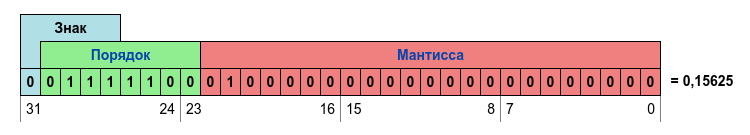
\includegraphics[width=0.9\linewidth]{\myFolder/1} \\
			Стандарт для хранения чисел с плавающей точкой. Можно почитать здесь: \href{https://ru.wikipedia.org/wiki/IEEE_754-2008}{вики}. \\
			Числа одинарной точности с плавающей запятой обеспечивают относительную точность 7-8 десятичных цифр в диапазоне от $ 10^{-38}$ до примерно $ 10^{38}$.
			Для вычисления показателя степени из восьмиразрядного поля порядка вычитается смещение порядка равное $127_{10} = 7F_{16} = 01111111_2$ (то есть, $01111100_2 - 01111111_2 = 124_{10} - 127_{10} = -3_{10}$). Так как в нормализованной двоичной мантиссе целая часть всегда равна единице, то в поле мантиссы записывается только её дробная часть. Для вычисления мантиссы к единице добавляется дробная часть мантиссы из 23-х разрядного поля дробной части мантиссы $1,01000000000000000000000_2$. Число равно произведению мантиссы со знаком на двойку в степени порядка = $1,01_2*2_{10}^{-3_{10}} = 101_2*2_{10}^{-5_{10}} = 5_{10}*2_{10}-5_{10} = 0,15625_{10}$. \\
			(Взято из \href{https://ru.wikipedia.org/wiki/%D0%A7%D0%B8%D1%81%D0%BB%D0%BE_%D0%BE%D0%B4%D0%B8%D0%BD%D0%B0%D1%80%D0%BD%D0%BE%D0%B9_%D1%82%D0%BE%D1%87%D0%BD%D0%BE%D1%81%D1%82%D0%B8}
				{другой статьи})
		\end{lecSubsection}
	\end{lecSection}
	\begin{lecSection}[Явное и неявное преобразование типов]
		\cppfile{\myFolder/2}{Неявное преобразование}{implicit_cast}
		В коде выше используется неявное преобразование: дает возможность писать код гибче, однако требует осторожнее (так, в строке 3 используется \textit{целочисленное} деление).
		\cppfile{\myFolder/3}{Не всегда удается преобразовать типы}{no_cast1}
	\end{lecSection}
	\begin{lecSection}[Типы целых чисел]
		В C++ есть несколько типов целых чисел:
		\begin{enumerate}
			\item \textbf{char} - код символа (по умолчанию 1 байт)
			\item \textbf{int} - целое число (сколько байт - не известно).
		\end{enumerate}
		Не стоит быть уверенным, что \textbf{char} - 1 байт, на разных процессорах по-разному. В C++ так устроено: язык заточен под процессор, на котором он будет выполняться. Для обоих типов можно указать \textbf{signed} и \textbf{unsigned} - знаковый тип или нет.
		\cppfile{\myFolder/sign_no_dec}{Пример доп. указателей к типам}{sign_no}. Стоит быть внимательным: сравнение для знаковых и беззнаковых может пойти не так, как хотелось бы. Пример:
		$-1 > 50$ - верное равенство, если -1 имеет тип \textbf{signed}, а 50 - \textbf{unsigned}. Проблема заключается в том, что $-1$ соответствует максимальному числу из \textbf{unsigned}.
	\end{lecSection}
	\begin{lecSection}[Логические операции]
		Работают над переменными типа \textbf{bool}.\\
		\begin{tabular}{cc}
			\multicolumn{1}{c|}{не} & $!A$ \\
			\multicolumn{1}{c|}{и} & $A\&\&B$ \\
			\multicolumn{1}{c|}{или} & $A || B$ \\
		\end{tabular}\\
		\vspace*{5pt}
		Здесь почти то же самое, что в Python, лишь синтаксис другой.
	\end{lecSection}
	\begin{lecSection}[Битовые операции C++]
		Как можно поменять две переменные без третьей? Для этого могут помочь логические операции. В C++ их несколько:
		\begin{enumerate}
			\item Инверсия -- $~x$ -- работает над \textit{любым} числом, не обязательно \textbf{bool}. Заменяет все ноли и единички в представлении числа на противоположные.
			\item Битовое \textbf{"и"} -- $x\& y$ -- умножает биты в двоичном представлении двух чисел. Иногда битовое "и" называют \textit{наложением маски}.
			\item Битовое \textbf{"или"} -- $x | y$ -- складывает биты в двоичном представлении двух чисел.
			% TODO: экранирование
			\item xor - x$\wedge$y. С его помощью можно как раз осуществить обмен переменных: \\
			x = x $\wedge$ y \\
			y = x $\wedge$ y \\
			x = x $\wedge$ y \\
		\end{enumerate}
	\end{lecSection}
	\begin{lecSection}[Автоматические типы переменных]
		\cppfile{\myFolder/auto}{Автоматический тип переменной}{auto}
		Код будет присваивать переменной х различные типы, однако этот трюк будет работать, только если компилятору сказать использовать современный стандарт (например, C++11)!
	\end{lecSection}
	
	\begin{lecSection}[Простейшие массивы]
		В C++, как и во многих языках, существуют массивы.
		\cppfile{\myFolder/array}{Пример объявления простейшего массива}{array}
		При объявлении массива надо указать его размер. По массиву можно итерироваться через обращение к элементу (точно так же, как в Питоне): A[1] -- второй элемент и так далее; нумерация идет с \textit{нуля}.\\
		 Подробнее о массивах будет рассказано на следующей лекции.
	\end{lecSection}
	
			\begin{center}
				{Исходные коды всех программ можно найти \href{https://github.com/alekseik1/cpp\_lections\_2017/tree/master/lection\%202}{здесь}}
			\end{center}
\end{lecture}
\stepcounter{lectureNo}

% TODO: ПОМЕНЯЙТЕ НА СВОЙ ПУТЬ ПРИ СБОРКЕ
\renewcommand{\mainFolder}{/home/aleksei/github_projects/latex_works/informatics/3sem}
\renewcommand{\myFolder}{\mainFolder/lecture_\arabic{lectureNo}/}

%	LECTURE INFO
%----------------------------------------------------------------------------------------
\renewcommand{\lectureSubject}{Адреса и указатели}
%----------------------------------------------------------------------------------------
%
% Главное - указывать в путях для добавляемых файлов переменную \myFolder.
% Так, новый cpp файл должен иметь путь \cppfile{\myFolder/main}{....} (указывается без расширения)
% Нельзя писать \cppfile{main}{...} !!!
% Если не выполнить это требование, большой проект не будет собираться


\begin{lecture}[\lectureSubject]
	\begin{lecSection}[Доступ к памяти]
		Память, выделяемая программе, неоднородна -- она делится на \textbf{сегменты}. Первый сегмент --- коды программы (режим "только чтение"). Второй -- сегмент DATA -- содержит данные программы. Более того, элементы DATA (к примеру, начальные значения переменных) записывается в .exe файл. Эти данные уходят в оперативку при запуске программы. Переменные, записанные в DATA, называются \textit{статическими}. Помимо этого, для функционирования программы необходима область \textit{стека} --- такой сегмент памяти, который заполнятся снизу вверх и изначально пуст. Когда ОС только загрузилась, в стек выделяется некоторое количество автоматической памяти -- для \textit{локальных переменных}. \\ 
		Память программе выделяется на время ее работы; после ее завершения память высвобождается.
		\cppfile{\myFolder/1}{Пример многократных вызовов функции}{1}
		Рассмотрим, как происходит работа с памятью в примере \ref{1}. Перед вызовом функции в стек программы будет выделено место для хранения "5" (оно в программе будет интерпретировано как n), stack pointer поднимается. stack pointer - это указатель, показывающий на текущее положение стека. Затем, после вызова функции, ее адрес возврата будет записан в стек - stack pointer двинется выше. Потом в стек уйдет "1" (мы же объявили ее). \\
		Попробуем написать функцию, считающую количество рекурсивных вызовов.
		\cppfile{\myFolder/2}{Функция для подсчета количества собственных вызовов}{2}
		Здесь k2 --- глобальная переменная. Ее присваивание происходит в \textit{момент компиляции} программы (т.е. она запишется в .exe и будет переноситься в память в момент загрузки). Функция \textbf{reducer} уменьшает значение k2. \\
		Однако глобальные переменные могут быть опасны! Считается, что нормальная функция не заглядывает в глобальные переменные (в таких случаях функцию называют "чистой", в противном - "грязной").
		\end{lecSection}
		\begin{lecSection}[Модификатор static]
		\cppfile{\myFolder/3}{Та же программа через static}{3}
		Мы переделали программу \ref{2}, теперь переменная k3 не видна в других блоках, но по-прежнему она записывается в сам .exe . Если бы функция была рекурсивной, то была бы такая ситуация, когда переменных k было бы много - на каждом слое рекурсии она создается. Они просто будут записаны в разные ячейки памяти и уйдут после того, как рекурсивный вызов завершится. 
		\cppfile{\myFolder/4}{Подсчет рекурсии}{4}
		В коде выше как раз \textbf{static} делает k одним для всех вызовов рекурсии --- оно при каждом вызове \underline{не} будет присваиваться в ноль. Вместо этого переменная будет увеличиваться на 1, таким образом, мы сможем увидеть глубину рекурсии.
	\end{lecSection}
	\begin{lecSection}[Указатель]
		Указатель - переменная адресного типа.
		\cppfile{\myFolder/5}{Адрес x можно указать}{5}
		Указатели тоже работают только со своими типами: в коде выше нельзя в \textbf{double*} записать число \textbf{int}. Дело в том, что возникнет ложная интерпретация -- ссылка на double превратися в ссылку на int, а поскольку в памяти double и int имеют разные размеры, то можно даже вылезти за пределы своей памяти. Компилятор это запретит, однако все можно обойти:
		\cppfile{\myFolder/6}{Пример обхода заперта}{6}
		У указателей могут тоже быть указатели:
		\cppfile{\myFolder/7}{Указатель на указатель}{7}
		Обратиться к переменной можно несколько способами:
		\cppfile{\myFolder/8}{Разница}{8}
		В последней строке происходит \textit{разыменование} адреса - грубо говоря, считывание данных из того адреса, куда указывает указатель. Разыменовывать надо последовательно:
		\cppfile{\myFolder/9}{Двойное разыменование}{9}
	\end{lecSection}
	\begin{lecSection}[Несколько слов о массивах]
		Массивов в C++ нет. Массив - это константный указатель на область памяти, представляющую содержимое!
		\cppfile{\myFolder/10}{Работа массива}{10}
		Команда объявления массива по факту означает следующее: создать n переменных типа int. \\
		С указателями можно прийти к \textit{адресной арифметике}: так, указатель $p+1$ выше означает, что мы сдвигаемся по памяти от места, куда указывает p, на \textbf{sizeof(1)}. Это иллюстрирует строка 7: A[i] абсолютно равносильна указателю *(A+i). Проверки на i \textit{нет}, то есть, в теории, мы можем убежать вообще в произвольную область памяти.
	\end{lecSection}
	\begin{lecSection}[Динамическая память]
		\cppfile{\myFolder/11}{Пример выделения из дин. памяти}{11}
		Динамическая память не является автоматической, т.е. ей надо явным образом указывать, когда ее выделять, а когда удалять. Если без конца писать вызов get(), то можно постоянно выбивать у системы память и это все приведет к \textit{memory leak} - утечке памяти.
	\end{lecSection}
	\begin{lecSection}[Передача параметров по указателю]
		Передача по параметрам бывает полезна, когда хочется поменять значение переменной внутри самой функции. Функции передается указатель и она, имея ссылку непосредственно на область памяти, может ее менять:
		\cppfile{\myFolder/12}{Передача указателей функции}{12}
		Подробнее -- в следующей лекции.
	\end{lecSection}
\end{lecture}
\stepcounter{lectureNo}

% TODO: ПОМЕНЯЙТЕ НА СВОЙ ПУТЬ ПРИ СБОРКЕ
\renewcommand{\mainFolder}{/home/aleksei/github_projects/latex_works/informatics/3sem}
\renewcommand{\myFolder}{\mainFolder/lecture_\arabic{lectureNo}/}

%	LECTURE INFO
%----------------------------------------------------------------------------------------
\renewcommand{\lectureSubject}{Динамическая память. Продолжение.}
%----------------------------------------------------------------------------------------
%
% Главное - указывать в путях для добавляемых файлов переменную \myFolder.
% Так, новый cpp файл должен иметь путь \cppfile{\myFolder/main}{....} (указывается без расширения)
% Нельзя писать \cppfile{main}{...} !!!
% Если не выполнить это требование, большой проект не будет собираться


\begin{lecture}[\lectureSubject]
	\begin{lecSection}[Динамические массивы]
		Как было сказано, массивов в C++ нет. Повторим объявление указателей: \\
		\cppfile{\myFolder/1}{Пример объявления указателей}{1}
		В строке \textbf{4} мы получаем указатель на \textbf{A[5]}. В строке \textbf{8} мы создаем число, да и еще присваиваем ему значение.
		\cppfile{\myFolder/2}{Объявление массива через \textbf{new}}{2}
		При объявлении массива через \textbf{new} нужно обязательно его удалять через \textbf{delete[]} -- оператор удаления.
	\end{lecSection}
	\begin{lecSection}[Структуры в C++]
		В C++ существует такая вещь, как структура -- набор переменных под одной крышей.
		\cppfile{\myFolder/ex1}{Простейшая структура}{ex1}
		Обратите внимание на строки \textbf{23} и \textbf{25}: такое сокращение еще часто будет встречаться (для указателей вместо "." используется "$->$"). Метод для распечатки мы вынесли отдельно для удобства. \\
		Подход к распечатке в самой первой функции имеет минус: при вызове функции мы создаем локальную копию Student. Метод \textbf{studentPrint1} лишен этого -- там передается по ссылке. Но возникает проблема, ведь мы внутри функции случайно можем изменить переменную x и этот результат будет виден извне. Решение дает передача по константной ссылке, что сделано в \textbf{studentPrint2}.\\ Существует еще одно решение задачи, в котором мы сначала создаем объект Student в памяти, получаем на него указатель, а затем через него меняем свойства объекта:
		\cppfile{\myFolder/ex2}{Еще одно решение со структурой}{ex2}
		Из структур можно составлять массивы, что неудивительно, учитывая, что массив - это просто несколько переменных. В качестве примера можно привести следующий код: \newpage
		\cppfile{\myFolder/ex3}{Массив из структур}{ex3}
	\end{lecSection}
	\begin{lecSection}[Массивы и функции]
		В функциях можно менять массивы, но их нельзя возвращать. Код внизу -- пример изменения массива внутри функции. \newpage
		\cppfile{\myFolder/ex4}{Изменение массива внутри функции}{ex4}
	\end{lecSection}
	\begin{lecSection}[Двумерный массив и передача его функции] 
		Двумерные массивы работают так же, как в Питоне. Тем не менее, у них есть некоторые особенности, связанные с их способом представления в памяти (помним, что массив по факту лишь набор переменных). Одна из этих особенностей видна в коде ниже, где мы передаем двумерный массив в функцию:
		\cppfile{\myFolder/ex5}{Передача массива в функцию}{ex5}
		Обратите внимание: в объявлении функции \textbf{printer} мы обязательно указываем длину (вторая квадратная скобка).
	\end{lecSection}
	\begin{lecSection}[Статические массивы]
		\cppfile{\myFolder/ex6}{Указание на элемент массива}{ex6}
		В коде выше видно, что для прохождения по элементам массива в функции  необходимо заранее знать его длину. Если посмотреть на выражение \ref{ex6}, то станет видно, что эта длина уходит в инструкции прохода по массиву еще на этапе компиляции, поэтому ее и нужно было передавать заранее, как это сделано в \ref{ex5}. Но можно ли сделать функцию \textbf{printer} без явного указания длины массива? Ответ дают динамические массивы.
	\end{lecSection}
	\begin{lecSection}[Динамические массивы]
		Динамические массивы --- это массивы, хранящиеся в так называемой динамической памяти (\textit{heap}). Динамические массивы объявлять несколько сложнее: так, для двумерного случая необходимо делать указатель на область памяти с указателями, каждый указатель в которой, в свою очередь, будет указывать на область памяти с нашими объектами (к примеру, \textbf{int}). Звучит не очень, однако пример \ref{ex8} может немного прояснить этот момент.
		\cppfile{\myFolder/ex7}{Объявление динамического массива}{ex7}
		\textbf{А} -- это массив из указателей типа \textbf{double*}. Каждый элемент этого массива - массив размера \textbf{width}. Таким образом, \textbf{А} есть двумерный массив. Обращение к его элементам происходит так же, как и при обычном объявлении массива, что видно в строке \textbf{26}.
		Мы сделали массив, распечатали его, а затем удалили, чтобы освободить память. При этом следует помнить такой трюк:
		\cppfile{\myFolder/ex8}{Порядок разыменования}{ex8}
	\end{lecSection}
		\begin{center}
			{Исходные коды всех программ можно найти \href{https://github.com/alekseik1/cpp\_lections\_2017/tree/master/lection\%204}{здесь}}
		\end{center}
\end{lecture}
\stepcounter{lectureNo}

% TODO: ПОМЕНЯЙТЕ НА СВОЙ ПУТЬ ПРИ СБОРКЕ
\renewcommand{\mainFolder}{/home/aleksei/github_projects/latex_works/informatics/3sem}
\renewcommand{\myFolder}{\mainFolder/lecture_\arabic{lectureNo}/}

%	LECTURE INFO
%----------------------------------------------------------------------------------------
\renewcommand{\lectureSubject}{Строки и файлы в C++}
%----------------------------------------------------------------------------------------
%
% Главное - указывать в путях для добавляемых файлов переменную \myFolder.
% Так, новый cpp файл должен иметь путь \cppfile{\myFolder/main}{....} (указывается без расширения)
% Нельзя писать \cppfile{main}{...} !!!
% Если не выполнить это требование, большой проект не будет собираться


\begin{lecture}[\lectureSubject]
	\begin{lecSection}[Хранение строк]
		Строки делятся на \textit{C-строки} и \textit{ANSI-строки}. В разных языках строки реализованы по-разному. Так, в Pascal они хранятся как \textit{ANSI-строки}: в первой ячейке памяти записана длина строки, а затем последовательно идут символы строки. Главный минус такого подхода --- ограниченность длины строки (255 символов). Этот недостаток отсутствует в \textit{C-строках}.
		
		В \textit{С-строках} используется следующая схема хранения: в памяти просто идет последовательность символов и завершается \textbf{нулем} (типа \textbf{int}, не "0"). Так, строка "Hello"\, будет записана как последовательность 'H', 'e', 'l', 'l', 'o', 0x0 (строки такого типа называются \textit{zero-ending string}). НО! Если мы сделаем обращение и изменим какой-либо символ на 0 (типа целочисленное), то строка поделится на две, ведь теперь у нее два символа окончания. Это --- один из минусов такого подхода.
	\end{lecSection}
	\begin{lecSection}[Операции со строками]
		Конкатенация строки можно делать с помощью стандартной библиотеки \textbf{cstring}.
		\cppfile{\myFolder/1}{Работа со строками}{1}
		В этом коде мы считываем строки, а затем их конкатенируем. Но Т.Ф. не любит эту библиотеку. Дело в том, что \textbf{strcat} сначала проходит и за линейное время находит ноль в конце строки, дабы узнать, где ее конец, а затем уже объединяет обе. Если такой код засунуть в цикл, то (из свойств арифметической прогрессии) мы подарим нашему коду квадратичную асимптотику.
		
		В MacOS сделано несколько интереснее: используется как число, равное длине строки, в ее начале, так и символ окончания в конце (комбинированный подход).
		
		При работе со строками следует быть осторожными: при операции \fbox{+=} можно уйти за аллоцированную (выделенную) память для данной строки и стереть ее содержимое. Кстати, в С++ строка --- это объект. Для нас сейчас это значит, что операции, которые нам кажутся простыми (наподобие \fbox{+=}), на деле такими не являются --- они реализованы по уму. К тому же, у строк есть свои методы и поля. К примеру, метод \textbf{s.size()} вернет длину строки за $O(1)$. У строк автоматическая работа с памяти --- язык автоматически выделяет столько памяти, сколько нужно.
		
		Т.Ф. рекомендует пользоваться C++ -- строками вместо С--строк.
	\end{lecSection}
	\begin{lecSection}[C++\, -- строки]
		В C++ строки входят в окружение \textbf{std}.
		\cppfile{\myFolder/2}{Объявление строки в С++}{2}
		В Python строки кодируются стандартом \underline{UTF-8}. В таком подходе память используется в разных количествах для разных символов, поэтому при вставке символа в середину строки возникают проблемы переноса (одна из причин, почему в Python строки неизменяемы). C++ лишен такого недостатка и здесь строку можно менять посимвольно.
		
		C++ не разделяет типы символа и \textit{кода} символа. Символ = код символа. Вообще, подробности можно изучить \href{http://cplusplus.com}{здесь}.
	\end{lecSection}
	
	\begin{lecSection}[Считывание строки]
		Существует несколько способов читать строки:
		\cppfile{\myFolder/3}{Считывание строки}{3}
		Обратите внимание: \textbf{cin $\gg$ s} возвращает \textbf{true} или \textbf{false}, в зависимости от того, закончился ли ввод.
		
		Другой способ заключался в методе \textbf{getline}, которому на вход поступает поток ввода (см. ниже) и строка s, куда будет записано. Различие следующее: \textbf{cin} читает до символа пробела, тогда как \textbf{getline} читает до символа переноса строки.
	\end{lecSection}
	\begin{lecSection}[Файловые потоки]
		Стандартная библиотека для работы с потоками --- это \textbf{fstream}. Она дает три потока для работы: \textbf{ifstream} для ввода и \textbf{ofstream} для вывода и \textbf{fstrim} для обоих вариантов.
		\cppfile{\myFolder/4}{Пример работы с потоками}{4}
		В коде выше было бы неплохо закрыть файл после окончания работы с ним. Более того, операционная система может дать отказ, если мы затребуем открытие слишком большого количества файлов. Однако C++ умный, он закроет файл после окончания существование объекта (в ходе выполнения деструктора, о них будет сказано в следующих лекциях).
		
		Во время открытия потока можно указать для него \textit{режим}: только для чтения и т.п.
		\cppfile{\myFolder/5}{Режимы потока}{5}
		Подробнее о режимах можно почитать в документации.
	\end{lecSection}	
	\begin{lecSection}[Строковые потоки]
		Работа со строковыми потоками тоже проходит через стандартную библиотеку:
		\cppfile{\myFolder/6}{Строковые потоки}{6}
	\end{lecSection}
	\begin{lecSection}[Односвязный список]
		Попробуем сделать односвязный список в C++ по аналогии с тем, что мы делали в Python.
		\cppfile{\myFolder/7}{Реализация односвязного списка}{7}
		\begin{enumerate}
			\item 		\textbf{typedef} --- это создание синонима типа \textbf{string}. Это сделано только для того, чтобы не писать каждый раз \textbf{std::string}, другого назначения у такой конструкции для нас нет.
			\item \textbf{struct tNode} --- объявление структуры ноды. В ней всего две переменные: свое значение и ссылка на следующую ноду.
			\item \textbf{tNode * \dots} --- сигнатура функции \textit{insert}\_\textit{node}. Ее мы опишем позже.
			\item В методе \textbf{main} мы создаем ноду через \textbf{new}, затем сохраняем ссылку на созданный объект. После этого мы записываем туда какую-то информацию ("Hello" в примере), далее прикрепляем к ней другие ноды.
			\item В цикле мы прогуливаемся по всем нодам и выводим их содержимое. Обратите внимание на переход к следующей ноде в последней строке цикла.
			\item Функция \textbf{insert\_node} --- изюминка нашего кода. Ей передается указатель на нашу ноду. Внутри функции мы создаем новую ноду, заполняем в нее данные из \textbf{data}, а в качестве следующей ноды записываем ту, что мы передали функции. Из этого получается, что мы добавляем ноды в обратном порядке, так как только что созданная нода встает впереди старой.
		\end{enumerate}
	\end{lecSection}
			\begin{center}
				{Исходные коды всех программ можно найти \href{https://github.com/alekseik1/cpp\_lections\_2017/tree/master/lection\%205}{здесь}}
			\end{center}
\end{lecture}
\stepcounter{lectureNo}

% TODO: ПОМЕНЯЙТЕ НА СВОЙ ПУТЬ ПРИ СБОРКЕ
\renewcommand{\mainFolder}{/home/aleksei/github_projects/latex_works/informatics/3sem}
\renewcommand{\myFolder}{\mainFolder/lecture_\arabic{lectureNo}/}

%	LECTURE INFO
%----------------------------------------------------------------------------------------
\renewcommand{\lectureSubject}{Продвинутая работа с функциями}
%----------------------------------------------------------------------------------------
%
% Главное - указывать в путях для добавляемых файлов переменную \myFolder.
% Так, новый cpp файл должен иметь путь \cppfile{\myFolder/main}{....} (указывается без расширения)
% Нельзя писать \cppfile{main}{...} !!!
% Если не выполнить это требование, большой проект не будет собираться



\begin{lecture}[\lectureSubject]
	\begin{lecSection}[Перегрузка (overload) функций]
		Полиморфизм --- много разных функций с одним именем. При вызове будет выбираться только одна: та, которая лучше всего подходит по входным параметрам. Это означает, что у функции один \textit{интерфейс} и много \textit{реализаций}. Рассмотрим пример:
		\cppfile{\myFolder/1}{Пример полиморфизма}{1}
		В примере \ref{1} мы пишем одну функцию \textbf{absolute} три раза: по одному на каждый тип входного (и, соответственно, возвращаемого) объекта. В случае, когда для заданного типа данных нет подходящей функции, C++ отбирает несколько функций как кандидатов на вызов, а затем выбирает их в следующем порядке:
		\begin{enumerate}
			\label{cand}
			\item Точное совпадение типов, если оно есть.
			\item Приведение путем повышения разрядности числа и вызов кандидата с полученным типом (например, \textbf{int8} $\rightarrow$ \textbf{int16})
			\item Стандартное приведение типов (например, \textbf{float} $\rightarrow$ \textbf{int}). Оно уже менее надежно, поэтому и находится ниже по приоритету.
			\item Пользовательское приведение типов, т.е. приведение к типу, объявленному пользователем (программистом, написавшим тип).
			\item Эллипсис. В C++ существуют функции, у которых на вход поступает неопределенное число параметров -- они называются эллипсис.
			\cppfile{\myFolder/2}{Пример эллипсиса}{2}
		\end{enumerate}
		Если на какой-то стадии проверки будет несколько кандидатов, равноправно удовлетворяющих условиям, то компилятор выдаст ошибку (он не поймет, какую вызывать).
	\end{lecSection}
	\begin{lecSection}[Шаблоны]
		Хотелось бы, чтобы можно было делать функцию с неопределенным типом, как здесь: \newpage
		\cppfile{\myFolder/3}{Неопределенный тип}{3}
		Однако C++ не позволит этого сделать. Дело в том, что при компиляции подобного кода необходимо под каждый тип переменной, для которой вызывается функция, иметь функцию под каждый из типов. В языке можно создать \textit{шаблон} и компилятор будет знать, как под каждый из них делать функцию. Исправим код:
		\cppfile{\myFolder/4}{Неопределенный тип с шаблоном}{4}
		Тут может возникнуть проблема. Если бы мы вызвали \textbf{absolute} от строки, то во время компиляции, при \textit{инстанцировании} функции для типа \textbf{string}, возникнет ошибка -- у \textbf{string} нет оператора унарного минуса (т.е. нельзя для строки s делать операцию `-s`). Эту проблему можно решить, если явно указать, каким типом инстанцировать функцию:
		\cppfile{\myFolder/5}{Явное инстанцирование функции}{5}
		Здесь мы изменили вызов на \textbf{absolute<int32\_t>}, тем самым указав тип, которым будет инстанцирована функция при компиляции.
		
		Посмотрим, как ведет себя шаблон:
		\cppfile{\myFolder/6}{Сложное инстанцирование}{6}
		В коде функция \textbf{self\_counter<1>} будет вызвана 3 раза, а \textbf{self\_counter<2>} -- только 2. Дело в том, что мы функцию инстанцируем по-разному: сначала с 1, потом с 2 (как будто это разные функции). Обратите внимание, в записи \textbf{template<int number>} подразумевается, что инстанцирование будет по числам, то есть при указании разных чисел инстанцируются разные функции. Простой код \textbf{self\_counter()} в этом случае уже не работает, так как для инстанцирования есть несколько подходящих кандидатов (см. \ref{cand}).
		\cppfile{\myFolder/7}{Инстанцирование с параметром по умолчанию}{7}
		Здесь мы уже задали значение по-умолчанию в шаблон (строка \textbf{3}), поэтому вызов без инстанцирования (строка \textbf{18}) сработал.
	\end{lecSection}
	\begin{lecSection}[Аргументы функции по умолчанию]
		В С++ можно создавать функции, у которых будут значения по умолчанию:
		
		\cppfile{\myFolder/8}{Функция с параметрами по умолчанию}{8}
	\end{lecSection}
	\begin{lecSection}[Односвязный список для любого типа данных]
		Пользуясь полученными знаниями, мы теперь мы можем переписать \textbf{LinkedList} из прошлой лекции:
		\cppfile{\myFolder/linkedList}{LinkedList}{9}
		Эту реализацию LinkedList можно несколько усложнить, разделив на файлы: один будет хранить лишь LinkedList, а другой будем пользоваться готовым кодом из первого. Получится что-то вроде библиотеки для Linked List. Часть ее реализации представлена ниже. Код далее достаточно сложен, и многие его аспекты будут объяснены в следующих лекциях.
		\cppfile{\myFolder/linkedListMain}{Основная часть}{10}
		\cppfile{\myFolder/linkedListHeader}{Хидер}{11}
		\begin{center}
			{Исходные коды всех программ можно найти \href{https://github.com/alekseik1/cpp\_lections\_2017/tree/master/lection\%206}{здесь}}
		\end{center}
	\end{lecSection}
\end{lecture}
\stepcounter{lectureNo}

% TODO: ПОМЕНЯЙТЕ НА СВОЙ ПУТЬ ПРИ СБОРКЕ
\renewcommand{\mainFolder}{/home/aleksei/github_projects/latex_works/informatics/3sem}
\renewcommand{\myFolder}{\mainFolder/lecture_\arabic{lectureNo}/}

%	LECTURE INFO
%----------------------------------------------------------------------------------------
\renewcommand{\lectureSubject}{Контейнеры в C++}
%----------------------------------------------------------------------------------------
%
% Главное - указывать в путях для добавляемых файлов переменную \myFolder.
% Так, новый cpp файл должен иметь путь \cppfile{\myFolder/main}{....} (указывается без расширения)
% Нельзя писать \cppfile{main}{...} !!!
% Если не выполнить это требование, большой проект не будет собираться



\begin{lecture}[\lectureSubject]
	\begin{lecSection}[LinkedList]
		Продолжим работу над кодом из предыдущей лекции:
		\cppfile{\myFolder/linkedList}{LinkedList}{1}
		\cppfile{\myFolder/linkedListHeader}{Header-файл для нашей программы}{2}
		Код заполнен не до конца, я не смог поспевать за Т.Ф. (если у кого будут исправления, прошу написать \href{https://vk.com/alekseik1}{мне}).
		\begin{center}
			{\large{ОБНОВЛЕНИЕ. Код всего проекта можно смотреть \href{https://github.com/alekseik1/cpp\_lections\_2017/tree/master/lection\%207}{здесь}.
			}}
		\end{center}
	\end{lecSection}
	\begin{lecSection}[Библиотека стандартных шаблонов С++]
		Библиотека стандартных шаблонов С++ называется \textbf{STL}.
		Она состоит из нескольких частей и типов, но выдерживает следующую структуру:
		\begin{enumerate}
			\item Контейнеры -- некоторый объект, содержащий данные.
			\item Итераторы -- позволяют \textit{итерироваться по элементам контейнера}.
			\item Алгоритмы -- название само говорит о предназначении. Примечательно, что они не имеют привязки к конкретному типу контейнера.
		\end{enumerate}
		\begin{tabular}{|p{0.31\linewidth}|p{0.31\linewidth}|p{0.31\linewidth}|}
			\multicolumn{3}{c}{\bfseries Таблица (для наглядности)} \\ \hline
			
			\hline Контейнеры	& Итераторы	& Алгоритмы \\	\hline
					Типы контейнеров: 
					\begin{enumerate}
						\item \textbf{vector<T>} (похож на \textbf{list} в Питоне)	
						\item \textbf{list<T>} (это \textbf{LinkedList} из Питона)
						\item 	\textbf{set<T>} -- красно-черное двоичное дерево поиска ($O(\log{N})$ - добавление/удаление/поиск.
						\item \textbf{unordered\_set<T>} -- хэш-таблица $O(1)$ -- добавление/удаление/поиск
						\item \textbf{map<T, V>} -- ассоциативный массив, состоящий из пар \textit{<key, value>}. При этом \textit{key} типа \textbf{T}, \textit{value} типа \textbf{V}
					\end{enumerate} &
					Типы итераторов:
					\begin{enumerate}
						\item \underline{input output} -- доступ к элементу содержимого контейнера по итератору
						\item \underline{bidirectional} $--$i -- если контейнер 'знает', что он двунаправленный
						\item \underline{random access} i = i + 100 -- итератор произвольного доступа (а не только по +1) 
						\item \underline{forward} ++i -- обычный шаг на один вперед
					\end{enumerate}  & \begin{enumerate}
					\item см. ниже 
				\end{enumerate} \\ \hline
		\end{tabular}
		\begin{lecSubsection}{Итерирование}
		Попробуем проитерироваться по контейнеру и применить к каждому элементу функцию \textbf{foobar}. Это можно сделать несколькими способами:
		\begin{enumerate}
			\item 		\cppfile{\myFolder/1}{Пример итерирования}{3}
			Здесь итератор \textbf{i} пробегает по всем значениям массива. Как он ведет учет текущей позиции, нас не волнует -- в этом и есть прелесть подобной структуры. Начало итерирования -- начало массива, конец итерирования -- конец массива. Есть и защита: если попытаться выйти за A.end() (например, на единицу), то при попытке разыменовать такой адрес выйдет ошибка. 
			\item 		То же самое итерирование можно было провести с помощью \textbf{foreach} (из библиотеки \textcolor{green}{\textbf{<algorithm>}})
			\cppfile{\myFolder/2}{Применение алгоритмов для итерирования}{4}
			Обратите внимание: функции \textbf{for\_each} уходит \textit{указатель} на функцию \textbf{foobar} (она ведь тоже хранится в памяти, как и переменные).
		\end{enumerate}

		В стандарте C++ 11 использование контейнеров упрощено:
		\cppfile{\myFolder/3}{Контейнеры в C++11}{5}
		Единственный минус: чтобы понять, что происходит в итераторе, приходится копать код вверх, до описания функции \textbf{foobar}.\\
		В примере \ref{5} используется \textbf{auto} -- автоматический выбор типа. При таком подходе компилятор сам подбирает подходящий тип для переменной.
		\end{lecSubsection}
	\end{lecSection}
\end{lecture}
\stepcounter{lectureNo}

% TODO: ПОМЕНЯЙТЕ НА СВОЙ ПУТЬ ПРИ СБОРКЕ
\renewcommand{\mainFolder}{/home/aleksei/github_projects/latex_works/informatics/3sem}
\renewcommand{\myFolder}{\mainFolder/lecture_\arabic{lectureNo}/}

%	LECTURE INFO
%----------------------------------------------------------------------------------------
\renewcommand{\lectureSubject}{Парадигмы программирования}
%----------------------------------------------------------------------------------------
%
% Главное - указывать в путях для добавляемых файлов переменную \myFolder.
% Так, новый cpp файл должен иметь путь \cppfile{\myFolder/main}{....} (указывается без расширения)
% Нельзя писать \cppfile{main}{...} !!!
% Если не выполнить это требование, большой проект не будет собираться



\begin{lecture}[\lectureSubject]
	\begin{lecSection}[Структурное программирование]
		Структурное программирование строится на следующей идее: разбивать сложную задачу на простые подзадачи. Достигается это путем решения подзадач в функциях. Таким подходом мы уже часто пользовались, но у него есть минус: со временем функций накапливается много и код становится менее читабельным.
		
	\end{lecSection}
	\begin{lecSection}[Модульное программирование]
		В качестве решения указанной проблемы можно функции собрать в отдельные \textit{модули}. Полученная парадигма носит название \textbf{модульного программирования}. Разумеется, при таком подход будет главный модуль -- к примеру, main.cpp. Главный модуль имеет одну особенность: в main.cpp есть функция \textbf{main}, которая содержит вход в программу. Таким образом достигается иерархия модулей.
		
		При построении взаимоотношений модулей очень важно правильно выстроить их зависимости. Нельзя допускать т.н. "межмодульную рекурсию": когда модуль \textbf{module1} инклюдит модуль \textbf{module2}, а модуль \textbf{module2} в то же время инклюдит модуль \textbf{module1}. Использование модулей заставляет думать об их организации.
		
		Стоит понимать, что все парадигмы нужны лишь для удобной воспринимаемости кода, но сами по себе они никак не ускоряют работы программ (а иногда даже могут и замедлить).
	\end{lecSection}
	\begin{lecSection}[Раздельная компиляция]
		Начнем с примера. Напишем структуру для дроби с возможностью использовать комплексные числа.
		%\cppfile{\myFolder/main}{main.cpp}{main1}
		%\cppfile{\myFolder/fractions.hpp}{fractions.hpp}{fractions.hpp}
		%\cppfile{\myFolder/fractions}{fractions.cpp}{fractions.cpp}
		%\cppfile{\myFolder/frac-complex.hpp}{frac\_complex.hpp}{frac\_complex.hpp}
		%\cppfile{\myFolder/frac-complex}{frac\_complex.cpp}{frac\_complex.cpp}
		Будем придерживаться следующей структуры:
		\begin{enumerate}
			\item \textbf{main.cpp} -- единица трансляции (то есть, компилируется). Подключает все хидеры. Собирается в \textbf{main.o}
			\item \textbf{fractions.hpp} -- хидер для \textbf{fractions.cpp}
			\item \textbf{fractions.cpp} -- единица трансляции (то есть, компилируется). Вместе со своим хидером собирается в \textbf{fractions.o}
			\item \textbf{frac\_complex.hpp} -- хидер для \textbf{frac\_complex.cpp}
			\item \textbf{frac\_complex.cpp} -- единица трансляции (то есть, компилируется). Подключает свой хидер \textbf{и} хидер \textbf{fractions.hpp} (потому что мы наверняка будем использовать его функции). При сборке соберется в \textbf{frac\_complex.o}.
		\end{enumerate}
		\begin{center}
			{\large{Код всего проекта можно смотреть \href{https://github.com/alekseik1/cpp_lections_2017/tree/master/lection%208}{здесь}.
				}}
		\end{center}
				
		Помимо прочего, наш проект может иметь несколько \textit{целей}: например, мы захотим собрать готовую программу или же тестовую; подключить файл-тестировщик или нет. Для этого применяется Makefile и система сборки \textbf{make}, однако она не будет обсуждаться в этой лекции. Если вас это заинтересовало, можете поискать в Гугле либо посмотреть исходники лекции, которую в данный момент читаете: она  собрана с использованием \textbf{make}.
		
		\begin{lecSubsection}{Разделяемые (динамические) библиотеки}
			Так называются библиотеки, которые содержатся в ОС. Распространяются в .dll в  ОС Windows или же .so в Linux.
		\end{lecSubsection}
		
		\begin{lecSubsection}{Отступление. Полезный материал на Фоксфорде}
		Подробности по С++ можно найти \href{https://foxford.ru/wiki/informatika/modulnoe-programmirovanie-v-c}{здесь} (материал достаточно ознакомительный, но из него можно вынести много полезного).
		\end{lecSubsection}
	
	\end{lecSection}
	\begin{lecSection}[Условная компиляция]
		Условная компиляция -- компиляция с условиями. Условия компилятору сообщают \textit{директивы} -- команды, обрабатываемые на этапе \textit{препроцессинга}. Часто используемая директива -- это \textbf{\#IFDEF}. Приведем пример ее использования:
		\cppfile{\myFolder/1}{Директива IFDEF}{1}
		Код в \underline{someCode} будет выполнен только тогда, когда был определен \underline{SOMETHING}. Существует похожая директива: \textbf{\#IFNDEF} -- только он срабатывает, если \textit{не} был определен аргументы.
		
		Еще один т.н. "страж включения": \textbf{\#define} \textbf{SOMETHING} -- объявляет \textbf{SOMETHING}. После него \textbf{\#ifdef} уже будет думать, что \textbf{SOMETHING} объявлено.
		
		Все эти штуки используются для того, чтобы не инклюдить один и тот же файл по несколько раз, ведь в таких ситуациях компилятор будет кидать ошибки.
	\end{lecSection}
	
	\begin{lecSection}[Макросы]
		\cppfile{\myFolder/2}{Пример использования макросов}{2}
		Макросы не рекомендуется использовать -- они создают обманчивую привлекательность, однако порождают непредвиденное поведение, поскольку \textbf{не} являются вызовами функции, а всего лишь подставляются препроцессором при текстовой обработке.
	\end{lecSection}
	\begin{lecSection}[extern-переменные]
		Представим себе, что мы хотим создать переменную, которая будет доступна и в том, и другом модуле. Можно ее описать в \textbf{main.cpp}, однако тогда нельзя будет ей пользоваться в тех файлах, которые не подключают \textbf{main.cpp}. 
		
		У нас есть \textbf{fractions.cpp}, которого все подключают. В нее запихнем эту переменную, а в \textbf{fraction.hpp} запишем \textbf{extern int g;}. Это скажет компилятору, что переменная \textbf{g} будет, но стоит ее дожидаться ТОЛЬКО во время компоновки (а не создавать каждый раз при \textbf{include}). То есть, все файлы, которые будут инклюдить \textbf{fractions.hpp}, будут иметь возможность обращаться к переменной \textbf{g}, но при этом сама переменная \textbf{g} будет объявлена \underline{только} в \textbf{fraction.cpp} (и никак не в файлах, которые индклюдят \textbf{fraction.hpp}). Это делает переменную \textbf{g} как глобальной, так и единой для всех файлов --- то, чего мы и добиваемся.
	\end{lecSection}
\end{lecture}
\stepcounter{lectureNo}

% TODO: ПОМЕНЯЙТЕ НА СВОЙ ПУТЬ ПРИ СБОРКЕ
\renewcommand{\mainFolder}{/home/aleksei/github_projects/latex_works/informatics/3sem}
\renewcommand{\myFolder}{\mainFolder/lecture_\arabic{lectureNo}/}

%	LECTURE INFO
%----------------------------------------------------------------------------------------
\renewcommand{\lectureSubject}{Объектно-ориентированное программирование}
%----------------------------------------------------------------------------------------
%
% Главное - указывать в путях для добавляемых файлов переменную \myFolder.
% Так, новый cpp файл должен иметь путь \cppfile{\myFolder/main}{....} (указывается без расширения)
% Нельзя писать \cppfile{main}{...} !!!
% Если не выполнить это требование, большой проект не будет собираться



\begin{lecture}[\lectureSubject]
	\begin{lecSection}[Класс]
		Класс --- это пользовательский тип, который объединяет данные и код, их обрабатывающий.
		
		Раньше мы `клали` данные структуры в объект \textbf{struct}, а рядом дописывали функции для нее. Теперь же мы хотим, чтобы с нашей структурой можно было работать \textbf{только} через функции, объявленные внутри нее. Этот принцип носит название \textit{принципа сокрытия данных}, а такая организация кода -- \textit{инкапсуляция}.
		\end{lecSection}
		
		\begin{lecSection}[Пример класса]
		Самый простой способ сделать подобие класса -- это использовать \textbf{struct}. Построим структуру \underline{Студент}, имеющую вид:
		\begin{enumerate}
			\item Поле \textbf{age} -- возраст студента
			\item Поле \textbf{name} -- имя
			\item Остальные методы, а именно:
			\begin{enumerate}
				\item \textbf{init} -- создание экземпляра
				\item \textbf{aging} -- увеличение возраста на 1
				\item \textbf{print} -- печать информации о студенте.
			\end{enumerate}
		\end{enumerate}
		
		\newpage
		\cppfile{\myFolder/1}{\textbf{struct} как пример класса}{1}
		В коде выше есть некоторые особенности:
		\begin{enumerate}
			\item Строка \underline{20} --- \textbf{const} после объявления функции означает, что внутри функции мы не можем менять сам объект класса.
			\item Строка \underline{31} -- не будет работать, так как "Vasya" есть \textbf{char[]*}, а метод класса требует \textbf{std::string}.
			\item Строка \underline{34} -- опасная операция (побитовое копирование может вести себя непредсказуемо, прим. ТФ).
			\item Мы можем изменять снаружи переменные \textit{внутри} объекта, то есть, имеет силу код \textbf{a.age += 10}. Это плохо, и дальше мы рассмотрим, как такую проблему решить.
		\end{enumerate}
	\end{lecSection}
	
	\begin{lecSection}[Конструкторы и деструкторы]
		\begin{lecSubsection}{Конструктор}
		Когда мы создавали объект `студент` в коде выше, нам каждый раз надо было инициализировать его через функцию \textbf{init()}. Однако мы можем это забыть сделать.
		
		Для защиты от этого существуют \underline{конструкторы} класса: особые методы, вызываемые при создании экземпляра класса. Перепишем код:
		\cppfile{\myFolder/2}{Наш класс с конструктором}{2}
		Конструктор ничего не возвращает. Помимо этого, объект класса \textbf{не} считается созданным до тех пор, пока не будет выполнен его конструктор.
		\end{lecSubsection}
		
		\begin{lecSubsection}{Деструктор}
		По аналогии с конструктором существует \textit{деструктор}.
		
		Деструктор --- особый метод, который ничего не возвращает и вызывается при удалении объекта.
		\end{lecSubsection}
		\begin{lecSubsection}{Конструктор по умолчанию}
			Если мы не создадим конструктор, то компилятор это сделает за нас, создав \textit{конструктор по умолчанию}. То же самое с деструктором.
			
			Однако, если мы создадим свой конструктор, то экземпляры класса уже надо будет клепать по его правилам, то есть, нам надо будет передавать объекту при создании те аргументы, которые принимает конструктор (в нашем случае \textbf{age} и \textbf{name}).
			\cppfile{\myFolder/3}{Особенности работы конструктора}{3}
			В примере выше на строке \underline{4} требуется вызов конструктора по умолчанию (при создании массива), а его нет -- поэтому она и помечена как неработающая. То же самое справедливо для строки \underline{1}.
			\newpage
		\end{lecSubsection}
		\begin{lecSection}[Примеры работы конструктора и деструктора]
			\cppfile{\myFolder/4}{Пример вызова деструктора}{4}
			В коде выше на строке \underline{12} мы делаем запись о том, что объект создан. На строке \underline{26} объявлен дестуктор -- код внутри будет выполнен, когда объект перестанет существовать.
			
			Код \ref{4} компилируется: попробуйте его запустить на своей машине и увидите, как работает деструктор.
		\end{lecSection}
		\begin{lecSection}[Пример. Структура Stack]
			\cppfile{\myFolder/5}{Структура Stack}{5}
			Обратите внимание на конструктор (строка \underline{7}) -- он может использоваться и как конструктор по-умолчанию (если не передавать ему параметры, так можно, когда есть значение параметра по умолчанию), и как свой (не дефолтный) конструктор (если передать параметр \textbf{max\_size}). В конце мы освобождаем ту память, которую занял объект \textbf{Stack}.
		\end{lecSection}
	\end{lecSection}
	\begin{center}
	Код всего проекта можно смотреть \href{https://github.com/alekseik1/cpp\_lections\_2017/tree/master/lection\%209}{здесь}.
	\end{center}
\end{lecture}
\stepcounter{lectureNo}

% TODO: ПОМЕНЯЙТЕ НА СВОЙ ПУТЬ ПРИ СБОРКЕ
\renewcommand{\mainFolder}{/home/aleksei/github_projects/latex_works/informatics/3sem}
\renewcommand{\myFolder}{\mainFolder/lecture_\arabic{lectureNo}/}

%	LECTURE INFO
%----------------------------------------------------------------------------------------
\renewcommand{\lectureSubject}{Инкапсуляция}
%----------------------------------------------------------------------------------------
%
% Главное - указывать в путях для добавляемых файлов переменную \myFolder.
% Так, новый cpp файл должен иметь путь \cppfile{\myFolder/main}{....} (указывается без расширения)
% Нельзя писать \cppfile{main}{...} !!!
% Если не выполнить это требование, большой проект не будет собираться



\begin{lecture}[\lectureSubject]
	\begin{lecSection}[Понятие инкапсуляции]
		В Питоне инкапсуляции не было. Когда мы делаем структуру, мы полагаем, что пользователь будет взаимодействовать с ней через те методы, что мы пропишем. Однако это может нарушиться. Для того, чтобы предотвратить такую ситуацию, существует \textit{инкапсуляция}. Инкапсуляция создает ограничения для программиста, тем самым организуя \textit{логику} нашего кода.
		\cppfile{\myFolder/1}{Инкапсуляция на примере класса Student}{1}
		В коде выше класс делится на две секции: \textbf{private} и \textbf{public}. То, что находится в секции \textbf{private}, \underline{не} будет видно снаружи класса. Эти секции могут следовать друг за другом в любом порядке и любом количестве(т.е., мы можем сначала описать публичную, потом приватную, затем опять публичную), но обычно их пишут один раз, объявляя сразу все, что нужно.
		
		Общий принцип инкапсуляции заключается в следующем: все атрибуты класса надо "прятать".
		
		При принятии решения, в какую из секций пихнуть свой метод, следует помнить, что \textit{конструкторы} класса \textbf{должны} быть публичными.
		
		\underline{Доп. инфа от ТФ.} Иногда может возникнуть необходимость разрешить создавать экземпляры класса, но не копировать их. В таких случаях конструктор класса следует сделать публичным, а конструктор клонирования положить в приватную секцию.
		\end{lecSection}
		
		\begin{lecSection}[Геттеры и сеттеры]
		
		При сокрытии полей стандартом обращения к ним служат \textit{геттеры} (getters) и \textit{сеттеры} (setters) -- методы, соответственно возвращающие и изменяющие поле. В нашем примере \ref{1} они объявлены на \textbf{13} и \textbf{18} строках.
		
		 Геттеры и сеттеры имеют интересную фишку: они не обязаны работать с существующим полем класса. Вполне возможно, что они будут задавать/возвращать другие величины, но пользователь будет думать, что они содержатся в классе. Так можно создавать удобные абстракции.
		
		\end{lecSection}
		
		\begin{lecSection}[Модификатор \textbf{const} после функции]
			В примере \ref{1} на строчке \textbf{25} мы видим модификатор \textbf{const} \textit{после} объявления метода. Это говорит компилятору, что метод не будет менять никаких полей класса в ходе своей работы. Стоит учесть, что если мы будем пользоваться константной ссылкой на экземпляр класса, то в ней мы сможем вызывать только константные методы (чтоб компилятор был уверен, что мы не изменим константный объект).
		\end{lecSection}
		
		\begin{lecSection}[Модификатор \textbf{static}]
			\begin{lecSubsection}{Статические поля}
				Иногда бывает необходимым сделать поле класса универсальным (т.е. единым) для всех его экземпляров. В таком случае используется модификатор \textbf{static}. Рассмотрим пример:
				\cppfile{\myFolder/2}{Простой пример статического поля}{2}
				Здесь мы при создании нового экземпляра класса увеличиваем \textbf{count} на 1, а при удалении -- уменьшаем. Важно отметить, что переменная \textbf{count} существует всегда, даже если не было создано ни одного объекта данного класса.
			\end{lecSubsection}
			\begin{lecSubsection}{Статические методы}
				Однако у такого подхода есть проблема: чтобы получить это поле через какой-либо метод класса, нам необходимо будет создать объект. Решает это, как можно догадаться, \textit{статический метод} (строка \textbf{12}). Такой метод привязан к классу, но никак не к объекту класса. Это несет свои минусы: статический метод не может в своем коде обращаться к нестатическим методам и полям (они ведь уже зависят от объекта, а статический метод от этого избавляется). Более того, в статическом методе \underline{не} определен \textbf{this} -- указатель на экземпляр класса.
			\end{lecSubsection}
			
			\begin{lecSubsection}{Пространство имен}
				В коде мы использовали (строка \textbf{32}) \textbf{SelfCounter} как \textit{пространство имен}. Каждый класс создает свое пространство имен, в котором находятся его поля и методы (разумеется, те, что в публичной секции). Таким способом удобно обращаться к статическим полям и методам.
			\end{lecSubsection}
		\end{lecSection}
		
		\begin{lecSection}[Дружественные функции]
			Бывает, что определенному классу \textbf{2} требуется добраться до атрибутов другого класса (класса \textbf{1}) (как это могут делать его экземпляры), но при этом сами классы никак не связаны. Для этого придется немного ослабить \textit{инкапсуляцию} и объявить в классе \textbf{1} (откуда хотим брать) требуемые \underline{дружественные} функции или даже классы. Затем дружественные функции или классы достаточно объявить где-нибудь снаружи -- и они уже будут иметь доступ внутрь \textbf{1}. Более того, можно сделать функцию дружественной даже в том случае, если она не была еще объявлена (предполагая, что это будет сделано позднее). При этом дружественные функции \textbf{не} являются методами класса \textbf{1} (того, куда мы открываем доступ).
			
			Иллюстрацией этому может служить следующий пример:
			\newpage
			\cppfile{\myFolder/3}{Пример дружественных функций}{3}
			В строке \textbf{1} мы объявляем класс \textbf{CarMaster}, но описываем его позже. Зачем?
			
			Если не объявить заранее CarMaster, то строка \textbf{8} будет вызывать ошибку, так как мы попытаемся обратиться к необъявленному классу. А объявить класс \textbf{CarMaster} перед \textbf{Car} мы не можем, так как в этом случае он будет обращаться к полю еще не объявленного класса \textbf{Car}. Решение этого -- описать сигнатуру класса \textbf{CarMaster} перед классом \textbf{Car}, но \textit{описать} ее позднее. Такой трюк мы будем часто использовать в будущем.
		\end{lecSection}
\end{lecture}
\stepcounter{lectureNo}

% TODO: ПОМЕНЯЙТЕ НА СВОЙ ПУТЬ ПРИ СБОРКЕ
\renewcommand{\mainFolder}{/home/aleksei/github_projects/latex_works/informatics/3sem}
\renewcommand{\myFolder}{\mainFolder/lecture_\arabic{lectureNo}/}

%	LECTURE INFO
%----------------------------------------------------------------------------------------
\renewcommand{\lectureSubject}{Наследование}
%----------------------------------------------------------------------------------------
%
% Главное - указывать в путях для добавляемых файлов переменную \myFolder.
% Так, новый cpp файл должен иметь путь \cppfile{\myFolder/main}{....} (указывается без расширения)
% Нельзя писать \cppfile{main}{...} !!!
% Если не выполнить это требование, большой проект не будет собираться



\begin{lecture}[\lectureSubject]
	\begin{lecSection}[Пример интерфейса -- UnivMan]
		Представим, что у нас есть некий шаблон, описывающий общую схему кода. Пусть это будет, к примеру, \textit{Unversity Man} -- для краткости будет звать его \textbf{UnivMan}. Им попробуем описать человека из МФТИ. Для нашего интерфейса сделаем некоторые методы: \textbf{getName()}, \textbf{getPhoto()}, \textbf{getDepartment()}. Их тело мы писать \underline{не} будем; эта работа ляжет на конкретную \textit{реализацию} нашего шаблона.
		
		Составим затем реализацию нашего шаблона: пусть, к примеру, мы захотим описать класс учителя вуза --- это класс \textbf{Teacher}. Создав этот класс, мы возьмем на себя обязанность реализовать \underline{все} методы, которые мы прописали в нашем 'шаблоне' \textbf{UnivMan}. При этом мы, помимо прочего, можем и дополнить наш 'дочерний' класс своими методами.
		
	\end{lecSection}
	\begin{lecSection}[Определение наследования]
		Такая иерархия классов подводит нас к третьей парадигме ООП: \textbf{наследованию}. Наследование --- это явление, когда один класс (потомок) перенимает все (строго говоря, почти все; о подробностях см. ниже) поля и методы другого класса (родителя).
		
		\underline{Замечание.} В нашем примере мы затребовали, чтобы класс \textbf{UnivMan} не содержал реализаций никаких функций. Такие классы называются \textit{интерфейсами} -- сами по себе эти штуки бесполезны, но они задают некий шаблон, по которому должны строиться его потомки (в примере это были \textbf{Teacher} и \textbf{Student}).
	\end{lecSection}
	\begin{lecSection}[Иерархия наследования]
		Вопрос о том, какой класс сделать родителем, а какой -- потомком, требует хорошей продуманности.
		
		Если бы мы хотели в нашем примере добавить класс \textit{старосты}, то его следовало бы сделать наследником класса \textit{студентов} и просто добавить специфичные методы (например, функцию раздачи задавальников). \underline{НЕ} стоит делать обычного \textit{студента} наследником \textit{старосты}, равно как и не стоит делать \textit{старосту} прямым наследником \textbf{UnivMan} и потом по-новой реализовывать те же самые методы, что \textit{студент} уже реализовал.
		
		Хорошим правилом для построения схемы наследования дает критерий Барбары Лисков: "Дочерний класс должен удовлетворять всем интерфейсам родительского класса \underline{и} не требовать ничего дополнительного."
	\end{lecSection}
	\begin{lecSection}[Модификаторы доступа]
		Для полей и методов можно разграничить права доступа: кто сможет их видеть, а кто нет. Для этого существует 3 модификатора доступа:
		\begin{enumerate}
			\item \textbf{public} -- доступно любым другим функциям (внутри класса, для потомков и остальных)
			\item \textbf{protected} -- доступно любым наследникам и самому классу.
			\item \textbf{private} -- доступно только самому классу.
		\end{enumerate}
		\cppfile{\myFolder/1}{Демонстрация модификаторов доступа}{1}
		Обратите внимание на строку \textbf{11} -- здесь слово \textbf{public} означает, что класс \textit{наследуется} публично. Другие куски кода будут знать, что \textbf{Derivative} наследует \textbf{Base} и мы сможем через объекты класса \textbf{Derivative} доступаться до всего, что есть в \textbf{Base}. В таком случае тоже можно делать разные модификаторы:
		\begin{enumerate}
			\item \textbf{public} -- все, кто имеет доступ к \textbf{Child} и \textbf{Parent}, будут знать о наследовании.
			\item \textbf{protected} -- только потомок и потомок потомка будут знать о наследовании. Поясним это. Путь наследование происходит по следующей схеме: $\textbf{Parent} \rightarrow \textbf{Child} \rightarrow \textbf{Child-of-child}$. При использовании \textbf{protected} в \textbf{Child} класс \textbf{Child-of-child} и только он будет знать о том, что \textbf{Child} унаследовал \textbf{Parent}. Потомки более высшего порядка и другие классы не будут знать о наследовании.
			\item \textbf{private} -- никто не будет знать о наследовании, кроме самого \textbf{Child}.
		\end{enumerate}
		Подробнее об этом можно прочитать \href{https://stackoverflow.com/questions/860339/difference-between-private-public-and-protected-inheritance}{здесь} (осторожно, английский!).
	\end{lecSection}
	\begin{lecSection}[Override -- переопределение методов]
		В дочернем классе мы можем не просто пользоваться методами родителя, а переопределять их. Это называется \textit{переопределением} метода.
		
		При этом есть и свои тонкости. Рассмотрим их на примере:
		\cppfile{\myFolder/2}{Тонкости вызова переопределенных функций}{2}
		Метод \textbf{foo} (строка \textbf{20}) 'видит' \textbf{x} как объект класса \textbf{Base}. И метод \textbf{b\_pub} он будет \underline{тоже} вызывать из этого класса, даже если мы \textbf{foo} на вход подадим экземпляр класса-наследника.
		
		Заметьте, что функцию мы могли бы и вызывать через обращение к классу как к пространству имен (строка \textbf{23}).
	\end{lecSection}
	\begin{lecSection}[Списки инициализации]
			С конструкторами бывают проблемы. Рассмотрим пример:
			\cppfile{\myFolder/3}{Тонкости конструкторов}{3}
			На строке \textbf{27} конструктор старосты. Ему \underline{нужно} вызвать конструктор родителя. Почему же?
			
			При создании объекта типа \textbf{ElderStudent} мы по факту берем класс \textbf{Student} и обертываем его тем, что мы написали в наследнике. Инициализация класса \textbf{Student} происходит через \textit{конструктор} класса \textbf{Student}. Таким образом, за счет наследования этого класса в \textbf{ElderStudent} мы заставляем программу выполнить конструктор родительского класса (\textbf{Student}). Но вызывать конструктор напрямую нельзя. Конечно, можно понадеяться, что компилятор сделает все тихо и в неявном виде, но что будет, если наш \textit{староста} в конструкторе будет получать не те переменные, что получал в конструкторе обычный \textit{студент}? А если у \textit{студента} нет конструктора по умолчанию, какой же тогда выбрать? Компилятор в этом случае не разберется и единственный способ разрулить ситуацию -- использовать \textit{списки 
				инициализации}. Это сделано после символа ':'.
			
			Магия списка инициализации заключается в том, что значение у нас будет инициализирован \textbf{Student} с параметрами \textbf{x} и \textbf{s} (их мы передали \textit{старосте} в конструктор) еще \underline{до} входа в само тело конструктора. Теперь у нас все хорошо: мы имеем инициализированного студента и уже готовы его отнаследовать и переопределять (что и сделано уже в \textit{теле} конструктора).
			
			Из вышесказанного вытекает \textit{важный вывод}: при создании объекта будут вызваны конструкторы \textbf{всех} родительских классов, начиная от самого старшего в иерархии.
			
			\begin{lecSubsection}{О порядке в списке инициализации}
			\textit{(Т.Ф. не успел этого рассказать на лекции)} При использовании списка инициализации можно инициализировать несколько переменных (а не только \textbf{Student(x, s)}, как у нас в примере). Важно то, что порядок инициализации \underline{не} будет зависеть от \underline{порядка перечисления через запятую} в нашем конструкторе, а будет целиком определяться порядком в \underline{исходном} классе. На нашем примере этого нельзя увидеть, потому что мы инициализируем лишь одну переменную, однако это будет заметно в следующем коде:
			\cppfile{\myFolder/4}{Маленький пример к порядку инициализации}{4}
			\end{lecSubsection}
			Порядок инициализации будет одинаков. Сначала в \textbf{age} уйдет 5, а затем в \textbf{mark} уйдет \textbf{age} (то есть 5). Кстати, в строке \textbf{5} видим еще один способ присвоить переменную \textbf{age} -- \textbf{age(5)}. Для \textbf{age} вызывается конструктор с параметром 5, от этого в \textbf{age} уйдет значение 5 (что логично). (Для тех, кто шарит: на примитивах этот трюк тоже работает. В С++ им для таких целей специально добавили конструктор)
		
	\end{lecSection}
\end{lecture}
\stepcounter{lectureNo}

% TODO: ПОМЕНЯЙТЕ НА СВОЙ ПУТЬ ПРИ СБОРКЕ
\renewcommand{\mainFolder}{/home/aleksei/github_projects/latex_works/informatics/3sem}
\renewcommand{\myFolder}{\mainFolder/lecture_\arabic{lectureNo}/}

%	LECTURE INFO
%----------------------------------------------------------------------------------------
\renewcommand{\lectureSubject}{Виртуальные методы}
%----------------------------------------------------------------------------------------
%
% Главное - указывать в путях для добавляемых файлов переменную \myFolder.
% Так, новый cpp файл должен иметь путь \cppfile{\myFolder/main}{....} (указывается без расширения)
% Нельзя писать \cppfile{main}{...} !!!
% Если не выполнить это требование, большой проект не будет собираться



\begin{lecture}[\lectureSubject]
	\begin{lecSection}[Вызовы методов при работе с классами-наследниками]
		Простейшие классы -- структуры. Напишем на них пример:
		\cppfile{\myFolder/1}{Пример виртуальных функций}{1}
		Заметьте, что у структур наследование всегда публичное.
		
		\begin{lecSubsection}{Распределение памяти}
			Экземпляр класса A будет занимать память, соответствующую размеру одного \textbf{char}'а, B -- уже одного \textbf{char} и одного \textbf{int} (для шарящих: пока пренебрежем выравниванием), С -- \textbf{int} и \textbf{double}. При этом занимаемые размеры расположатся в таком порядке: $ a < b < c $.
		\end{lecSubsection}
	
		\begin{lecSection}[Виртуальные методы]
			Рассмотрим пример:
			\cppfile{\myFolder/2}{Вызов наследника вместо родителя}{2}
			Какая функция будет вызвана в \textbf{foo()}? Ответ прост: всегда из класса \textbf{A}. Дело в том, что функция \textbf{foo} \textit{компилируема}: при сборке проекта \textbf{p} будет 'увиден' компилятором как экземпляр класса \textbf{A} и вызов \textbf{p.bar()} будет привязан к области памяти \textbf{A}.
			
			Как бороться с этим? Есть несколько способов:
			\begin{enumerate}
				\item Поле типа (\underline{не рекомендуется}). Добавим специальный атрибут \textbf{int m\_type} в базовый класс. В конструкторах производных классов заполним \textbf{m\_type} своими ID типа (например, у \textbf{A} будет 0, у \textbf{B} будет 1). При этом будет происходить \textit{коммутация} вызовов:
				
				\textbf{p.bar()} превратится вот в такое:
				\cppfile{\myFolder/3}{Условия на поле типа}{3}
				Это кошмар. Нам надо знать все классы, которые наследуют базовый, да и к тому же вести их учет через ID. Есть альтернатива.
				\item Сохраним указатель на функцию в классе. Она уйдет всем наследникам. В конструкторе каждого наследника мы будем переопределять ссылку на этот метод, вот так:
				\cppfile{\myFolder/4}{Переопределение указателя на функцию}{4}
				Остаются проблемы. Вдруг дочерний класс будет использовать родительский метод? Вдруг таких методов будет много? Приведем еще один способ.
				
				\item \label{v3} Можно хранить не одну ссылку на метод, а указатель на таблицы, содержащей указатели на нужные методы. Те же костыли, те же проблемы. Запутаться еще легче, ведь для каждого класса эта таблица будет своя.
			\end{enumerate}
			
			Но есть и  хороший способ. Все это уже встроено в язык. Все обрабатывается \underline{автоматически}. Для этого нужно только одно -- указать перед методом слово \textbf{virtual}. Для всех потомков будет создана таблица виртуальных методов (подобно той, что указана в п.\ref{v3} выше), которая будет автоматически заполняться у потомков.
			
			Итак, \textit{виртуальные} методы -- те методы, которые предполагаются быть переопределенными в дочерних классах.
		\end{lecSection}
		
		\begin{lecSection}[Множественное наследование]
			\begin{lecSubsection}{Абстрактный класс}
				Класс, у которого есть хотя бы один абстрактный метод с нулевой реализацией, является \textbf{абстрактным}. Его экземпляры нельзя создавать, но при этом абстрактные классы обладают мощной штукой -- множественное наследование.
				\cppfile{\myFolder/5}{Абстрактный метод с нулевой реализацией}{5}
			\end{lecSubsection}
			\begin{lecSubsection}{Множественное наследование}
				Множественное наследование --- это явление, когда один класс наследует несколько других. При этом класс, как это говорят, будет удовлетворять нескольким \textit{интерфейсам}. У такой штуки есть масса проблем. Что, если оба класса имеют два одинаковых метода с одинаковой сигнатурой? А атрибуты? С ними могут возникнуть большие проблемы при пересечении. Но если все методы виртуальны, а атрибутов нет, то все славно: даже если классы содержат пересекающиеся методы, мы сможем выбрать для переопределения любой из них (компилятору будет все равно, ведь они все равно не содержат реализации). Именно поэтому рекомендуется делать множественное наследование \underline{только} в абстрактных классах и наследовать при этом \underline{только} абстрактные классы.
			\end{lecSubsection}
			
			\begin{lecSubsection}{Применение абстрактных классов}
				Итак, в чем польза абстрактных методов и классов? Они позволяют грамотнее и логичнее организовывать структуру кода, объединяя схожие классы. Наглядный пример их использования мы видели в лабе 12 'Арифметические драконы', когда реализовывали класс \textbf{Dragon}, а впоследствии и класс \textbf{Enemy} -- каждый из них не обозначал какой-либо реальный объект сам по себе, однако служил шаблоном для клепания других классов, уже вполне связанных с реальными объектами (например, \textbf{Dragon} служил образом для класса \textbf{GreenDragon}).
			\end{lecSubsection}
		\end{lecSection}
	\end{lecSection}
\end{lecture}
\stepcounter{lectureNo}

% TODO: ПОМЕНЯЙТЕ НА СВОЙ ПУТЬ ПРИ СБОРКЕ
\renewcommand{\mainFolder}{/home/aleksei/github_projects/latex_works/informatics/3sem}
\renewcommand{\myFolder}{\mainFolder/lecture_\arabic{lectureNo}/}

%	LECTURE INFO
%----------------------------------------------------------------------------------------
\renewcommand{\lectureSubject}{Исключения в С++}
%----------------------------------------------------------------------------------------
%
% Главное - указывать в путях для добавляемых файлов переменную \myFolder.
% Так, новый cpp файл должен иметь путь \cppfile{\myFolder/main}{....} (указывается без расширения)
% Нельзя писать \cppfile{main}{...} !!!
% Если не выполнить это требование, большой проект не будет собираться



\begin{lecture}[\lectureSubject]
	\begin{lecSection}[Понятие исключения]
		Пусть некая функция \textbf{main()} вызывает функции \textbf{A,B,C,D} по схеме $A\rightarrow B\rightarrow C\rightarrow D$. Что произойдет, если одна из них не сможет выполнить свои обязательства (встретится какая-нибудь ошибка, ресурсы будут недоступны и т.п.)?
		\begin{lecSubsection}{Интерфейс функции}
			Прежде чем ответить на этот вопрос, разберемся с таким понятием, как \textit{интерфейс функции}. Интерфейс функции -- это некий абстрактный набор, содержащий характеризующую функцию информацию. Он включает \textit{имя, смысл, типы параметров, их допустимые значения и \underline{возможные} исключения}. Интерфейс функции должен быть продуман перед разработкой, на этапе осмысливания архитектуры целого приложения.
		\end{lecSubsection}
	\end{lecSection}
	\begin{lecSection}[Исключения в С++]
		\label{exc1}
		В С++, как и во многих языках программирования, наша ошибка выполнения будет обработана следующим образом: неисправная функция создаст \textbf{исключение} и вернет вызвавшей ее функции это исключение. Та, с свою очередь, должна будет его обработать дальше. Исключения, порождаемые функцией, являются самостоятельными типами. Они имеют свои поля и атрибуты.
	\end{lecSection}
	\begin{lecSection}[Стек вызова]
			Когда одна функция вызывает другую, вторая отправляется в \textit{стек вызовов}. Это такая очередь, содержащая функции в том порядке, в каком они вызывались. В стеке лежат функции и \textit{адреса возврата} -- адрес того места функции в оперативной памяти, где была вызвана новая функция (чтобы впоследствии вернуться строго в то место, где выполнения программы прервались на вызов другой функции). Помимо адресов в стек вызовов уходят локальные переменные, место для аргументов функции, место для возвращаемого значения (или для адреса, если возвращаемое значение лежит в динамической памяти). При этом передаваемые аргументы будут передаваться по обычным правилам (с использованием конструктора копирования для объектов и т.п.).
	\end{lecSection}
	\begin{lecSection}[Порядок вылета из программы]
		Что произойдет, если вылетит исключение и не будет обработано? Программа вылетит, причем весь код дальше выполнен \underline{не} будет. Это может привести к утечке памяти (если мы таким способом пропустим \textbf{delete}, освобождающий память) и другим проблемам (о них ниже).
	\end{lecSection}
	\begin{lecSection}[Реализация исключений в С++]
		Теперь посмотрим, какова реализация механизма исключений в С++. Работа с опасным кодом в этом языке осуществляется следующим образом:
		\cppfile{\myFolder/1}{Синтаксис исключений}{1}
		При этом \textbf{ExceptionType} -- это тип исключения (см. \ref{exc1}). Если в опасный код выбросит исключение типа \textbf{ExceptionType}, то программа начнет выполнять код в блоке \textbf{catch}. Если это исключение другого типа, оно \underline{не} будет обработано.
	\end{lecSection}
	\begin{lecSection}[Проблемы исключений]
		В процессе 'вылета' из-за исключения остальные объекты нашей программы будут удалены. А для этого нужно вызвать их деструкторы. Что произойдет, если при этом деструктор сам выбросит исключение, не знает даже Т.Ф., поэтому деструкторы надо писать максимально простыми и \underline{не} выбрасывающими исключения.
		
		Еще одна проблема, которая может случиться -- исключение во время выполнения конструктора. При таком исходе объект не будет до конца создан и для него не будет вызван деструктор. Это тоже может вести к утечкам памяти.
	\end{lecSection}
	\begin{lecSection}[Иерархия исключений]
		Сами исключения, как объекты классов, имеют свою иерархию. Самое базовое исключение есть экземпляр класса \textbf{BaseException}. От него наследуются уже специфичные исключения, например, \textbf{ArithmeticException} -- исключение в арифметике (деление на ноль и т.п.). Все эти типы можно передать в \textbf{catch}, тем самым указав типа ошибки, который будет обработан в конкретном блоке.
		\begin{lecSubsection}{Default exception}
			Исключение вида:
			\cppfile{\myFolder/3}{Default exception}{3}
			является исключением по умолчанию. Это, по-простому говоря, исключение на все случаи жизни. Т.Ф. не рекомендует им пользоваться, ведь этот тип практически ничего не будет знать о деталях ошибки.
		\end{lecSubsection}
	\end{lecSection}
	\begin{lecSection}[Вторичные исключения]
		При обработке исключения в блоке \textbf{catch} может случиться такое, что с какими-то проблемами наш блок будет в состоянии разобраться, а с какими-то -- нет. В последнем случае \textbf{catch} может сам выкинуть exception и передать его уже выше. Это делается командой \textbf{throw}.
		\cppfile{\myFolder/2}{Пример вторичного исключения}{2}
	\end{lecSection}
\end{lecture}
\stepcounter{lectureNo}

